\documentclass[authoryear, review,12pt,number]{elsarticle}
%\documentclass[authoryear, preprint,12pt,number]{elsarticle}
\usepackage[utf8]{inputenc}
\usepackage[T1]{fontenc}
\usepackage[numbers]{natbib}
\usepackage{graphicx}
\usepackage{float}
\usepackage{rotating}
\usepackage{stfloats}
\usepackage{lineno}
%\usepackage[linesnumbered,ruled,vlined]{algorithm2e}
\usepackage{tabulary}
\usepackage{graphicx}
\usepackage{color}
\usepackage[none]{hyphenat} \usepackage[table]{xcolor} \sloppy
\usepackage{hyperref}
\usepackage{amsmath}
\usepackage{multirow}
\usepackage{rotating}
\usepackage{adjustbox}
\usepackage{graphicx}% http://ctan.org/pkg/graphicx
\usepackage{booktabs}% http://ctan.org/pkg/booktabs
\usepackage{xparse}% http://ctan.org/pkg/xparse
\usepackage{booktabs}
\usepackage{array}
\usepackage[ddmmyyyy]{datetime}
\usepackage{listings}

\renewcommand{\dateseparator}{.}

\newcolumntype{R}[2]{%
    >{\adjustbox{angle=#1,lap=\width-(#2)}\bgroup}%
    l%
    <{\egroup}%
}
\newcommand*\rot{\multicolumn{1}{R{60}{1em}}}% no optional argument here,
% please!
\begin{document}
\begin{titlepage}
\begin{center}

% Upper part of the page. The '~' is needed because \\
% only works if a paragraph has started.
\textsc{\LARGE Technische Universit\"at Berlin}\\[0.5cm]
\textsc{Master Thesis}\\[1.5cm]

\textsc{\Large Classifying EUNIS Habitats using Ontologies and Data Mining
Methods}\\[1.5cm]
\textsc{\textit{A thesis submitted in partial fulfillment of the requirements
for the degree of}}\\[1.25cm]
\textsc{\Large Master of Science in Environmental Planning}\\[1.5cm]
\textsc{Faculty VI - Planning Building Environment\\
 Geoinformation in Environmental Planning}\\[1.5cm]

% Title
% Author and supervisor
\noindent
\begin{minipage}{0.5\textwidth}
\begin{flushleft} \large
\emph{Author:}\\
T. Niklas \textsc{Moran}
\end{flushleft}
\end{minipage}%
\begin{minipage}{0.5\textwidth}
\begin{flushright} \large
\emph{Supervisor:} \\
Prof. Dr.~Birgit \textsc{Kleinschmit}
Mag. rer. nat. ~Simon \textsc{Nieland}
\end{flushright}
\end{minipage}

\vfill

% Bottom of the page
{\large December 2015}

\end{center}
\end{titlepage}

\begin{titlepage}
\begin{center}
{Author's Declaration}
\end{center}
I hereby certify that I am the sole author of this master thesis. 
Furthermore, I confirm that no sources have been used in the preparation of this thesis other
than those indicated in the thesis itself. The works of other people included in
my thesis, published or otherwise, are fully acknowledged in accordance with the
standard referencing practices. This thesis has not been submitted for another
degree or master to any other University or Institution.
\\
\\
Hiermit versichere
ich, dass ich die vorliegende Arbeit selbstst�ndig verfasst und keine anderen als die
angegebenen Quellen und Hilfsmittel benutzt habe. Alle Ausf�hrungen, die anderen
ver�ffentlichten oder nicht ver�ffentlichten Schriften w�rtlich oder
sinngem\"a\ss entnommen wurden, habe ich kenntlich gemacht. Die Arbeit hat in
gleicher oder \"ahnlicher Fassung noch keiner anderen Pr\"ufungsbeh\"orde vorgelegen.

\vfill
\begin{center}
\noindent
\begin{minipage}{0.5\textwidth}
\begin{flushleft}
\rule{5cm}{0.4pt}
Date/Datum 
\end{flushleft}
\end{minipage}%
\begin{minipage}{0.5\textwidth}
\begin{flushright} 
\rule{5cm}{0.4pt}
Signature/Unterschrift
\end{flushright}
\end{minipage}


\end{center}
\end{titlepage}
%\pagebreak
\begin{center}{\textbf{Introduction to Master's Thesis}}\end{center}
Humans depend on well-functioning ecosystems for survival and have
recognized as such in a number of nature conservation laws and treaties such
as the Convention on Biological Diversity(CBD). The European Union has
implemented the Habitats Directive (Council Directive) 92/43/EEC [1992] to
comply with the CBD and protect biodiversity in the EU. As part of the
directive, periodic reports detailing status need to be submitted every six
years. The true potential of the directive is not yet realized as the data
in the reports is difficult to compare due to varying data collection
methods and aquisition nomenclatures. The differing collection methods of
member states when performing field surveys, which are already subjective,
compounds the problem (Cherrill 199). Luckily, with remote sensing data,
Geographic Object Based Image Analysis (GEOBIA) and ontologies stored as
OWL2/XML files, these biodiversity reports could become cheaper, more
objective and less time consuming.

This Master's Thesis presents a method for a semi-automatic ontology-based
classification system that has been applied to formalized EUNIS dry, mesic,
wet (E1, E2, E3) grasslands in Saarburg, Rhineland-Palatinate. I have chosen
to write this thesis in the form of a scientific journal article to
disseminate my findings in the hopes that it might be useful to someone
else. In the pages that follow is the soon to be submitted journal article. At 
the end of the article are links to the OWL ontologies.

\begin{center}{\textbf{Zusaammenfassung}}\end{center}
Die Fernerkundung ist entscheidend f\"ur das Biodiversit\"at-Monitoring. Sie 
hilft die Anforderungen von bestehenden Gesetzen, wie z.B. der 
EU-Habitatrichtlinie, zu erf\"ullen. Voll eingesetzt bringt sie die 
M\"oglichkeit, in der Zukunft eine Vielfalt von aufkommenden Herausforderungen 
zu \"uberwinden und etwaige Probleme zu l\"osen. Trotz dieser 
positiven Attribute ist das volle Potenzial der Fernerkundung jedoch noch nicht 
realisiert, weil verschiedene Begriffe und Klassifikationssystem in 
Biodiversit\"at-Monitoring gewendet wird. Ergebnisse zu Vergleichen ist nicht 
einfach, Daten-austauschen gleich so und Fragen von Herkunft/Herangehensweisen 
sind offen. Au\sserdem sind Feldmesskampagnen subjektiv, teuer und 
arbeitsaufwendig. Automatisierten Software und Methoden die Nachvollziehbare, 
Vergleichbare und Objektive Ergebnisse liefern ist n\"otig. Diese Probleme sind 
in einen Semi-Automatisierten Ontologie-basierte-Klassifikation die Data 
Mining Algorithmen verwendete um empirische Klassifikationergebnisse auszugeben. 
Die Methode wurde in Saarburg, Rheinland Pfalz an EUNIS Grasland Biotopen 
verwendet und einen ersten schritt um einen Automatisierten 
Biodiversit\"ats-Monitoring System zu realisieren. 

\begin{center}{\textbf{Acknowledgements}}\end{center}
This thesis would not be possible without the help of Simon Nieland and the 
NATFLO project. I thank Simon for all his patience, guidance and for leading me 
to this great field of research. I would like to thank Professor 
Dr. Birgit Kleinschmit for her feedback and the opportunity to work in her lab; 
as without it this thesis would not exist. I would like to thank all of my 
colleagues for a great work environment and rewarding collaboration.
\lstset{language=XML}

\begin{frontmatter}
\linenumbers
\title{Classifying EUNIS habitats using ontologies and data mining methods}

\author[TUB]{T. Niklas Moran\corref{cor1}}
\ead{niklasmoran@mailbox.tu-berlin.de}

\author[TUB]{Simon Nieland}
\author[TUB]{Birgit Kleinschmit}

\address[TUB]{Geoinformation in Environmental Planning Lab, Technische
Universit\"at Berlin, Stra\ss e des 17. Juni 145, 10623 Berlin, Germany}

\cortext[cor1]{Corresponding author at: Geoinformation in Environmental Planning
Lab, Technische Universit\"at Berlin, Stra\ss e des 17. Juni 145, 10623 Berlin,
Germany}

\begin{abstract}
Biodiversity monitoring using remote sensing is critical in order to 
meet future challenges and existing laws such as the EU Habitats Directive. The 
subjective nature of field surveys, conducted to meet reporting guidelines of  
the Habitats Directive, combined with differing nomenclatures and procedures 
of EU member state environmental agencies hampers data exchange and comparison. 
Furthermore, manual field surveys are expensive and time-consuming. To meet 
these future challenges automated tools are needed to use remote 
sensing data to produce comparable, empirical data outputs that lend 
themselves to data discovery and provenance needs. These requirements describes 
a developed semi-automatic ontology-based, multi-source EUNIS classification 
method that is tested on a region in Rhineland-Palatinate, Germany. 
\end{abstract}

\begin{keyword}
remote sensing, biotope classification, data mining, nature conservation, OWL, 
EUNIS, GEOBIA
\end{keyword}
\end{frontmatter}
\linenumbers

\section{Introduction}
Recognizing the importance of functioning ecosystems to reduce biodiversity 
loss, the European Union has implemented an environmental conservation 
framework to protect and conserve vital habitats in accordance with the 
Convention on Biological Diversity. An integral part of this framework is the 
EU Habitats Directive (Council Directive) 92/43/EEC [1992], which established 
the Natura 2000 network of habitats. The directive requires conservation and 
monitoring of designated habitats by member states and for a report to be 
submitted every six years. Environmental data to determine biodiversity status 
must be collected to comply with the statute. Yet, comparing data used for 
these reports is difficult due to varying data collection methods and 
acquisition nomenclatures by the nature conservation authorities in each member 
state \citep{VandenBorre2011}. The main issue lies in the subjective nature of 
field surveys to identify habitats \citep{Cherrill1999, Cherrill1999a, 
Hearn_2011, Nieland2015}. Furthermore, habitat status is mostly generated in 
bottom-up approaches taking into account the national and regional 
interpretation guidelines \citep{VandenBorre2011, INSPIREdataspecs}. This 
subjective and time-consuming task of conducting field surveys could be 
partially replaced with an automated remote sensing (RS) method that uses 
Geographic Object-Based Image
Analysis(GEOBIA) to reduce subjectivity, costs and time.

Remote sensing offers opportunities to collect and automatically interpret large
amounts of computer-readable data useful for nature conservation and
biodiversity monitoring \citep{Corbane2015, VandenBorre2011, Mayer2011}. RS
image analysis implicitly incorporates the expertise of the person performing
the analysis, reducing reproducibility as the analyst ultimately chooses class
membership in non-crisp boundaries between classes. This can be divided into
remote sensing knowledge (spectral signature, remote sensing indices, etc.) and
field knowledge (feature properties, spatial relations, etc)
\citep{Andres2013a}, which is often neither completely nor explicitly defined as
it is based on trial and error but influences the classification
\citep{Arvor2013}. To ensure accuracy and applicability of classification
outputs for conservation, experts with detailed knowledge of the sites are
needed to interpret the RS data. The distance between the high-level semantics
used by experts to describe domain concepts and the low-level information
quantified from data is referred to as the ``semantic gap''.

Ontologies can help bridge the ``semantic gap'' and allow for better data
transferability, predictability, interchangeability, knowledge and workflow
management (provenance) and logical consistency \citep{Janowicz2012}.  The
standards-compliant format designed and adopted to express rich semantics and
enable the ``Semantic Web'' is called the Web Ontology Language
(OWL2)\footnote{\url{http://www.w3.org/TR/owl2-overview/}}. The format supports
multiple syntaxes yet defines the Resource Description Framework (RDF)/XML
(subject, predicate, object triplets) as a common exchange format.  Moreover,
through the use of reasoners (inference engines) that infer logical consequences
over axioms and asserted facts and verify consistency, one can discover new
knowledge \citep{Arvor2013, Andres2013a}

RS and field expert knowledge can be digitized in ontologies, thus allowing for
a hierarchy of concepts for improved automatic image annotation and retrieval
using concepts from both fields to produce more accurate results
\citep{Srikanth_2005}. Janowicz \cite{Janowicz2012} advocates for more
observation-driven ontologies and for including machine learning, statistics and
data mining to construct ontological primitives. While published research on
using observation-based ontologies for biotope classifications is limited, the
available research using ontologies in RS research is briefly summarized below.

Ontologies modeled on the Land Cover Classification System and the General
Habitat Category were integrated into tools used to monitor and protect areas in
the EU \citep{Arvor2013}. The authors note that using the taxonomy of the
different classification systems makes it possible to include expert knowledge
in the process. \cite{Lucas2015} used pixel-based analysis and OBIA for greater
classification accuracy which relies on a rule-base created by an expert. Other
research includes classification of urban building types using a three-layered
architecture \citep{diSciascio2013} and a semi-automated classification of urban
building using the Random Forest (RF) classifier to determine variable
importance of features from airborne laser scanner data \citep{Belgiu2014}.
Ontologies have also been paired with different algorithms to automatically
acquire classification rules: a genetic programming algorithm
\citep{Forestier2012470} and the C4.5 data mining algorithm
\citep{Sheeren2006ML}. In biodiversity monitoring research, ontologies have been
demonstrated to improve spatial data interoperability by \cite{Nieland2015} and
a habitat quality tool showing trends and indicators led to the discovery of
relationships between phenomena \citep{Perez-Luque2015}.  The addition of fuzzy
data types to OWL2 and the development of a fuzzy spatial reasoner holds great
promise for the future of GEOBIA ontology research using remote sensing
\citep{Bobillo2011, Bobillo2015}. More recently a multi-scale fuzzy spatial
reasoner was developed which could have significant impact on this research
\citep{Argyridis2015}.

Even though researchers recently developed a number of indicators using
different sensors for habitat evaluation \citep{Nagendra2013}, classification
procedures and rule-sets were not formalized to be computer readable and
therefore suffer from similar transferablity and reproducibility problems as
manual habitat mapping \citep{Arvor2013, Nieland2015}. Therefore a formalized
computer-readable ontology could help solve these problems and allow scientists
to see how the classification was performed and be aware of possible
incompatibilities before combining data \citep{Janowicz2012}.  Furthermore,
there is no standardized set of indicators using RS for trans-national habitat
evaluation \citep{Lucas2015, VandenBorre2011}. Therefore, technical solutions to
increase interoperability by thematically harmonizing environmental data and
systematize data collection methods from remote sensing inputs in an automated
workflow are needed. 

The EIONET Action Group on Land monitoring in Europe (EAGLE) is an expert group
that seeks to harmonize land cover (LC) and land use (LU) nomenclatures using an
object-oriented data model that eases translations between nomenclatures
\citep{arnold2013eagle}. The many different nomenclatures used in Europe each
have their own specific thematic conceptualization suited towards a specific
scale and data collection method- reducing the ability to compare thematic maps.
Since LU and LC are interconnected and influence one another, nomenclatures
often incorporate both definitions into one class making separation difficult.
To overcome this problem the EAGLE data model describes landscapes in three main
components: land cover (abiotic, vegetation, water) land use (agriculture,
forestry, etc.) and characteristics (bio-physical, cultivation etc). The
increased interoperability and transferability of RS data and the semantic layer
on top helps decision-makers to better assess and compare outcomes. 
% The goal is to produce what Janowicz describes as a
% ``micro theory'' \citep{Janowicz2012} which can then be used to map other theories
% by training the data mining algorithms for the new region and using the
% reasoner. We hope that once good test sites are taken for a region (for instance
% the federal state of Rhineland Palatinate) that the data mining algorithms will
% identify rules for ontological primitives that captures the concept well using
% RS and other environmental data, negating the need to re-train. This speeds
% up classification and makes generation of new reference data unnecessary. This
% refers especially to the ones, which are derived from rather stable data sources
% like the indices of the DEM/DSM.

In this paper we propose an automated system that can classify dry, mesic and
wet grassland habitats according to the European Union Nature Information System
(EUNIS) biotope classification schema using earth observation data, existing
thematic maps (biotope, forestry, etc.), and expert knowledge formalized in an
ontology by taking into account rules generated by data mining algorithms. The
combination of data mining algorithms with ontology-based classification has, to
our knowledge, not yet been done and is a first in remote sensing research.
This method contributes to the goal of empirically-derived rule creation and
enhances data interoperability and comparison as proposed \cite{Janowicz2012}.
The main goals of this paper are:
\begin{itemize}
 \item to develop a RS classification methodology using data mining approaches
     in combination with ontological formalism to generate highly interoperable,
     reproducable and exchangeable classification procedures and results,
 \item apply the methodology to indicators used to separate grassland habitats
     defined under EUNIS
 \item and evaluate the developed approach by comparing it to a state-of-the art
     machine learning classifier (Extra Tree 
Classifier 
\footnote{\url{
http://scikit-learn.org/stable/modules/ensemble.html#extremely-randomized-trees
}}).
\end{itemize}
\section{Use case: Classifying EUNIS grasslands in Rhineland-Palatinate}
\label{sec:usecase_data}
To test the feasibility of applying our method to a real-world use case, we 
tested our method on dry, mesic and wet grasslands (EUNIS E1, E2 and E3 
respectively) in the district of Saarburg within the federal state of 
Rhineland-Palatinate (RLP). 
Saarburg is an 200km$^{2}$ administrative district and is located in the
south-west of the federal state of Rhineland Palatinate (RLP), Germany.
Luxembourg borders the area to the west and the federal state of Saarland to
the South. RLP has a western european atlantic climate and has an economically
and culturally important viticulture industry along the Mosel and Rhine rivers.
\begin{figure}
\label{fig:study_area}
    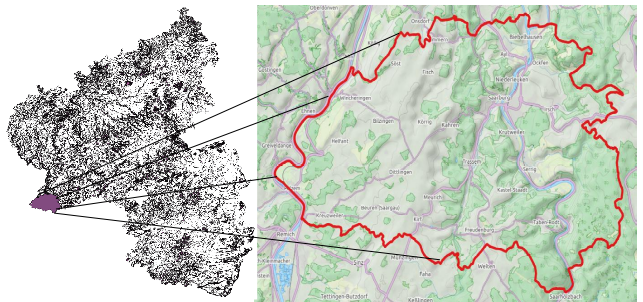
\includegraphics[width=\textwidth]{diagrams/study_area_closeup.png}
    \caption{The location of Saarburg (in purple) in relation to
    Rheinland-Palatinate. Map on right \copyright Thunderforest, Data\copyright
    OpenStreetMap contributors.}
\end{figure}
We adapted the selected EUNIS indicators to meet the requirements of remote
sensing analysis. We also adopted EAGLE's object-oriented approach by separating
land use, land cover and characteristics (biophysical and anthropogenic) and
adopted terms when possible to increase interoperability and further re-use.
The table ~\ref{tab:indicators_classes} shows the list of indicators that can be
detected by our data and aggregated to form EUNIS classes. 
\begin{table}
\centering
  \begin{tabular}{clcccccccc}
  \rot{description}&\rot{EUNIS class}&\rot{wetness} & \rot{vegetation type} &
  \rot{usage} & \rot{usage intensity} & \rot{immature
  soil} & \rot{hydromorphic} & \rot{species richness} \\ \hline
\multirow{3}{*}{dry}
    & E1   & dry & g/h & g/m/- & low & 1 & 0 & 0/1/- \\ 
    & E1.2 & dry & g/h & g/m/- & low & 1 & 0 & 1\\
    & E1.7 & dry & g/h & - & low & 1 & 0 & -/0\\ 
\multirow{4}{*}{mesic} 
    & E2   & mesic & g/h & g/m/- & l/m/h/- & 0 & 0 & 0/1/-\\
    & E2.1 & mesic & g/h & g & medium/high & 0 & 0 & -/0/1 \\
    & E2.6 & mesic & g & g/m/- & high & 0 & 0 & 0 \\
    & E2.7 & mesic & g/h & - & - & 0 & 0 & 0/1/- \\
\multirow{3}{*}{wet}
    & E3   & very wet & g/h & g/m/- & low/medium & 0 & 1 & 0/1/- \\
    & E3.4 & very wet & g/h & g/m & medium & 0 & 1 & 0/1 \\
    & E3.41 & very wet & g/h & m & medium & 0 & 1 & 1 \\
\end{tabular}
\caption{A `/ ' denotes OR and a '-' denotes 'none' and the first letter of 
each value is used to safe space. Vegetation type: {graminaceous, 
herbaceous}, usage: {grazing, mowing}, usage intensity: {low, medium, high}. 
}
\label{tab:indicators_classes}
\end{table}
\label{subsec:segmentation}
\subsection{Segmentation}
For the pre-segmentation step two types of data were taken into account. 
Digital orthophotos (resolution 0.2m) are used to create the Digital Surface 
Model (DSM) (resolution 0.5m) using automated stereo matching and therefore 
represent the basis for all segmentation and classification procedures. The DTM 
and DEM was produced using LiDAR ASCII point clouds acquired between 2003 and 
2009 with a resolution of 0.2m.\\ The reference
data (see \ref{subsec:reference_data_and_semantic_characterisation})
consists of the federal biotope map (partially updated 2015), agricultural data
updated every year and a soil map (resolution xxx) which is based on the ALKIS 
(Amtliches Liegenschaftskaster Informationssystem- Automated Land 
Registration Map) The actual classification process is based on two RapidEye 
Scenes (Year:xx and yy) and indices of the DTM, DEM and orthophotos.

\begin{figure} 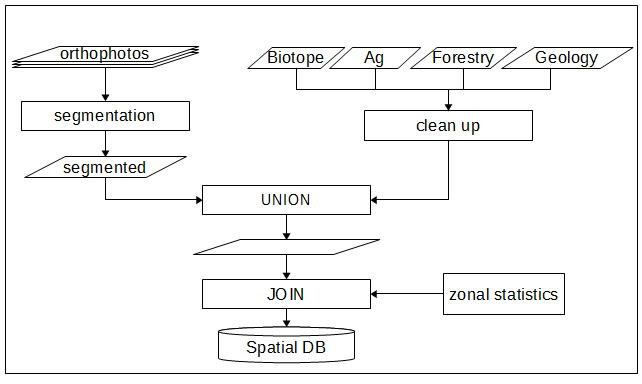
\includegraphics[width=1\textwidth]{diagrams/pre_processing.png}
    \caption{biotope, agriculture and soil maps are combined 
    (union) and joined with the segmented polygons (derived from orthophotos) 
    fitting within the combined polygons. The features are joined together 
    and all properties associated from the data are appended unless they 
    conflict. 
    When conflicts occur the corresponding column is marked as such.}
\label{fig:pre-processing}
\end{figure}
\section{Method}
This section describes the developed ontology-based, multi-source EUNIS 
habitat classification method.
\label{subsec:method_overview}
\subsection{Overview of the automated EUNIS Habitat Mapping System}
Figure ~\ref{fig:full_workflow} gives an overview of the method using the
wetness indicator as an example of one of the habitat indicators needed to
differentiate dry, mesic and wet grassland habitats according to level 2 of
EUNIS. The developed system is comprised of (1) the preparation of reference
data, including a spatial union of the base data sets (pre-segmented,
pre-classified areal photos and thematic maps (see 
\ref{subsec:reference_data_and_semantic_characterisation}) and the
attachment of subsequent semantic characteristics (see 
\ref{subsec:LU_anthropomorphic}),
(2) the selection of training and validation data (see
\ref{subsec:Selection_of_training_validation_data}
the generation of classification rules using machine learning algorithms and
finally (4) the ontology-based classification process (see
\ref{subsec:Onto_classification}}).
The software relies on a PostgreSQL database and various open source Python and
Java libraries to interact with the database, convert files and execute a
reasoner over the created OWL file. The OWLAPI
\footnote{https://github.com/owlcs/owlapi} is used to interact with the
OWL files and execute the FaCT++ reasoner \citep{Tsarkov2006}. Currently the
rule generation module uses two algorithms: decision tree classifier (DT) and
one additional algorithm called the Separability and Thresholds (SEaTH)
algorithm \citep{Nussbaum2006}. The extra trees classifier (ET) is used as a
reference classification.
\begin{figure}
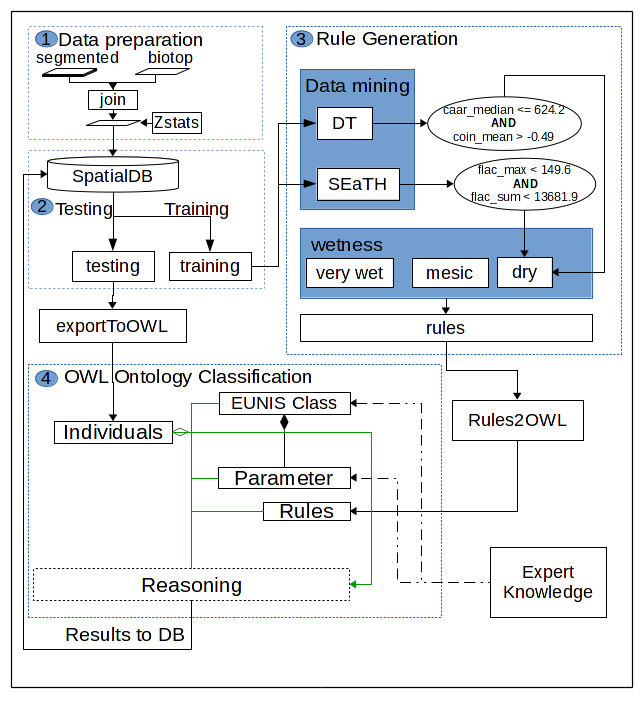
\includegraphics[width=1\linewidth]{diagrams/final_workflow_diagram.png}
\caption
    {
        1) The thematic maps (biotope, soil, etc.) are unioned together and
        statistics are calculated for each combined polygon.
        2) Training and testing data are created and saved in the database.
        3) The rules are generated for e.g.\ the ``wetness'' indicator from
        training data.
        4) The rules are imported into the OWL ontology along with the testing
        data as individuals. The reasoner performs A-box reasoning to determine
        class membership.
    } 
\label{fig:full_workflow}
\end{figure}
\label{subsec:reference_data_and_semantic_characterisation} 
\subsection{Reference data preparation semantic characterization}
The iterative object-based image analysis is performed by \cite{Tintrup2015} 
using Defiens eCognition Server in a multi-resolution approach 
\citep{baatz2001ecognition} taking into account thresholds. The data is 
segmented by multi-spectral (B, G, R, NIR) orthophotos (see 
\ref{sec:usecase_data}) spectral information and indices (Bare Area Index, 
etc.) and height from the DEM to separate between biotic and abiotic features 
\citep{Tintrup2015}. The detailed data preparation workflow is shown in figure 
\ref{fig:pre-processing}. This segmentation follows the EAGLE concept and
captures land cover classes and labels created polygons as such. This step is
crucial as the quality of the segmentation determines the quality of the later
identification step as the value of an indicator such as wetness for a grassland
might differ for that of a forest. Using EUNIS class descriptions and
interpretation guidelines \citep{EUNISManual}, a set of indicators tailored to
the available input data for our test area were created. Detailed analysis of
the EUNIS nomenclature showed that some indicators do not lend themselves to
easily be detected by RS data. Therefore consulting with an expert ecologist,
indicators were added to produce a meaningful formalization of the classes. The
formalization can be written to an OWL ontology, which is able to store complex
logical connections (axioms) in an OWL2 file.

An OWL2 ontology is composed of classes, individuals and properties. Classes are
sets of individuals and properties come in two forms: an object property defines
a relationship between two individuals and a data property  places a data type
constraint on the individual \citep{OWL2}. Furthermore, a reasoner can perform
A-Box and T-Box reasoning over the defined axioms. 

Relationships between objects (subsumption, disjointedness, etc). are discovered
and checked for consistency during T-box reasoning. Using software, such as
Protege, users can see how the defined axioms are related in the stored
knowledge base (OWL2) and check for logical consistency. If OWLIndividuals
(objects) are in the knowledge base then A-Box reasoning can also be performed
finding if any of the individuals fit into the defined classes. As EUNIS is an
hierarchically structured classification scheme testing that the formalization
follows the same hierarchy is important. 

\subsubsection{Land cover extraction and biophysical characteristics}
\label{subsec:LC_biophysical}
We use environmental variables (e.g., wetness, soil maturity, vegetation type,
etc.) from the classification schemes and concepts from EAGLE to preserve
interoperability by using this well-formalized vocabulary. All used indicators
for this research are shown in Table \ref{tab:indicators_classes} An example of
a EUNIS class, E2.22 ``Sub-Atlantic lowland hay meadows'' modelled with selected
remote sensing indicators is written in description logic (DL) below
~\ref{eq:description_logic}.

Land cover extraction is performed by the segmentation process documented in 
section \ref{subsec:segmentation}.  These polygons include spectral information 
and various statistics and indices such as SAGA wetness index, wind effect, 
etc. This follows the EAGLE data model's separation of LU and LC information.

\subsubsection{Land use and anthropomorphic characteristics}
\label{subsec:LU_anthropomorphic}
We combined agricultural, foresty, biotope and geological data from different
sources, creating a comprehensive database for Rhineland Palatinate. These
thematic maps have anthropomorphic characteristics of the land use such as
cultivation and management practice (grazing or mowing). These polygons are much
larger than the polygons produced by the segmentation (see
\ref{subsec:reference_data_and_semantic_characterisation}, so
that all polygons completely within the thematically combined polygon receives
all of its attributes. This step adds the class labels used for training the
data mining algorithm. 
\begin{equation}
\begin{align*}
%\begin{split}
    E2.22 &\equiv \exists has\_wetness \{``mesic''\} \\
    &\qquad {} \cap \exists has\_hydromorphic \{``false''\} \\
    &\qquad {} \cap \exists has\_immature\_soil \{``false''\} \\
    &\qquad {} \cap \exists species\_richness \{``false''\} \\
    &\qquad {} \cap \exists has\_usage \{``mowing''\} \\
    &\qquad {} \cap \exists has\_usage\_intensity \{``medium''\} \\
\end{align*}
\label{eq:description_logic}
\end{equation}
\label{subsec:Selection_of_training_validation_data}
\subsection{Selection of training and validation data}
\subsubsection{SeATH}
Training the SEaTH algorithm starts with 15 objects per class being randomly 
selected from the training data. One benefit of the SeATH algorithm is that one 
does not need many training objects. In \cite{Nussbaum2006}, for example, the 
authors suggest using only very characteristic features for training and only 
used around 10 samples per class. The authors also state that usually two 
features per class is enough to produce accurate results.
\subsubsection{DT and ET}
We use an evolutionary search algorithm with 10 evolutions based on the 
Distributed Evolutionary Algorithms in Python \citep{DEAP_JMLR2012} software to 
find the best features and used balanced class weights due to the very 
different distribution of grassland biotopes.  Three different fitted DT 
classifiers were compared: 1) a DT fitted with the features chosen by the 
evolutionary search algorithm 2) a DT trained on all features with parameters 
chosen after trial and error 3) a DT trained on the top 10 most important 
features as chosen by the ET classifier. Each DT classifier undergoes a 5-fold 
cross validation to verify results and the highest overall accuracy DT is 
chosen.
\label{subsec:rulegen_data_mining}
\subsection{Rule generation}
For the DT case the tree is parsed according to the depth first search
algorithm. Starting with the root node, the algorithm visits edges first, 
traveling as far as and only when it reaches a leaf node does it backtrack. The 
nodes contain the decision thresholds and all nodes visited before reaching the 
leaf node (the parents of that node) are chained with AND together to create a 
rule. The leaf node also has information on how many objects were classified by 
going down this branch and how many were falsely classified. The rule is 
assigned to the class with the best accuracy at that leaf node. The process 
continues until all leaf nodes are visited. The rules are joined 
together by logical ORs and become a rule set for the indicator under 
investigation. An example decision tree trained on immature soil is depicted in 
\ref{fig:decisiontree}.
\begin{figure}
    \label{fig:decisiontree}
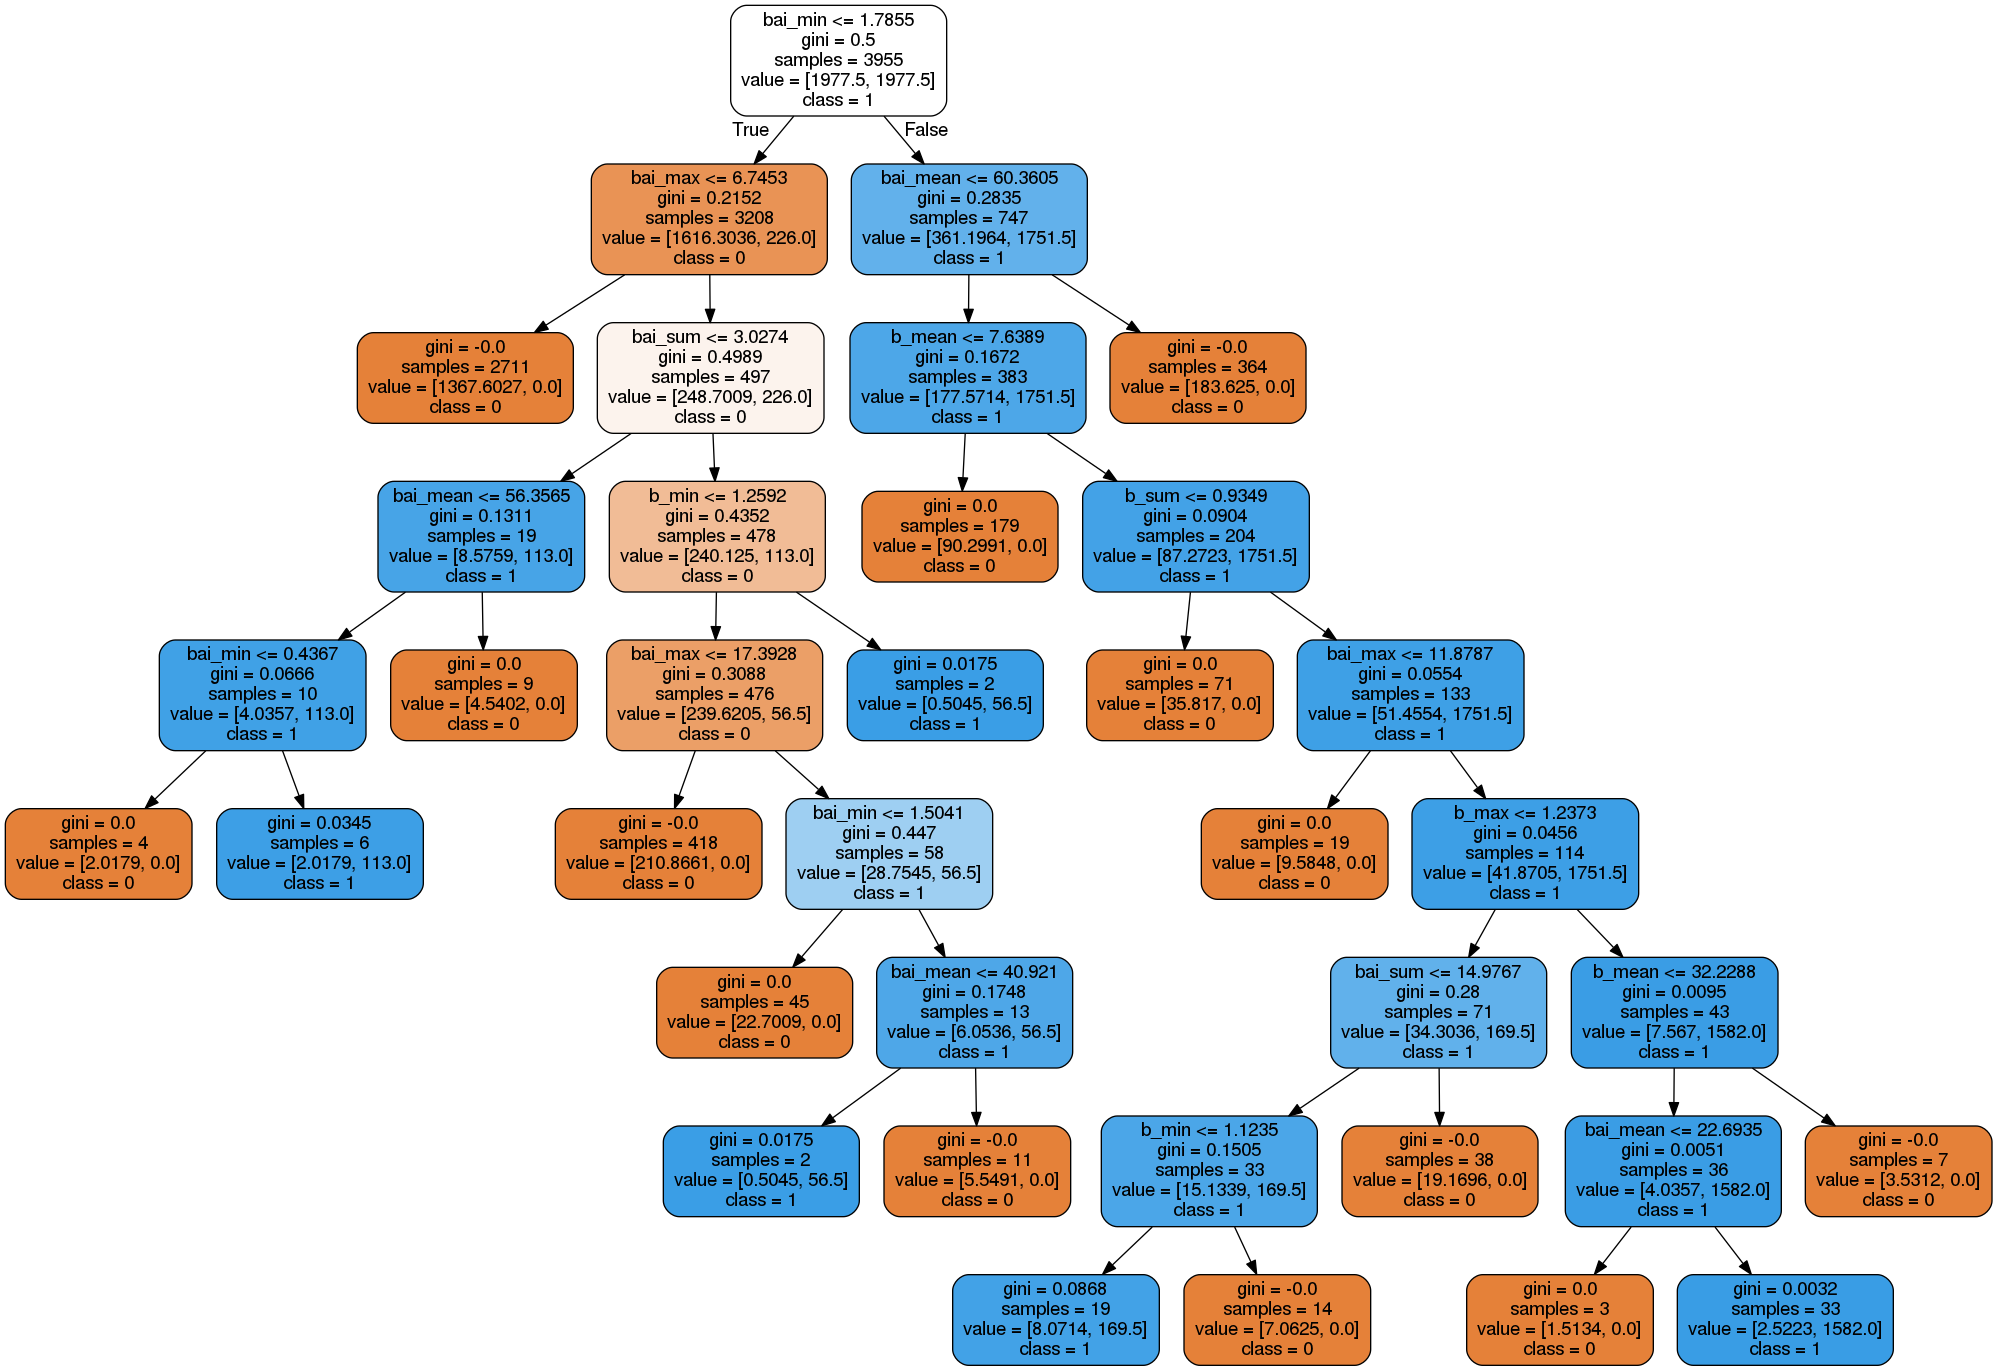
\includegraphics[width=\textwidth]{diagrams/natfo_immature_soil_dt.png}
    \caption{An example decision tree trained on immature soil indicator}
\end{figure}
The SEaTH algorithm outputs rules that include the best features to separate 
one class from another. Since we have over 200 features and the authors of 
SEaTH suggest using only 2-3 features, we parse the first three lines as the 
list is sorted from best to worst. We join the features with their 
corresponding thresholds using logical ANDs. We do this for every class, 
chaining the preceding rule and the next rule with an OR. An example rule from 
the DT is shown below.
\\
The subclass ``low'' from ``usage intensity'' has a rule that is generated by
the decision tree algorithm as seen in \ref{lst:dt_rule_snippet_csv} below. 
The first name is the feature/statistic's name, followed by a threshold. For 
the DT, as in the example, the last number is the node in the tree where the 
threshold comes from. This information is currently not being used.
\label{lst:dt_rule_snippet_csv}
\begin{lstlisting}
    wief_max,>,1.092550,0
    tpi5_max,<=,-0.341000,420
    swi_median,<=,8.097600,421
    toin_max,<=,1536.561279,422
    pan4_glcm_std_135,<=,-7.890923,423
    b_std,<=,10.100981,424
\end{lstlisting}
\ref{lst:dt_rule_snippet_owl} shows how the first two 
lines of this rule look in an OWL2/XML ontology. The rule has a collection of 
DataSomeValuesFrom within a nested datatype restriction corresponding to the 
rule threshold. A class can be defined by many rules containing multiple 
datatype properties that are chained together with logical AND (intersection) 
operators. The rules are then joined by a logical OR operator as can be seen in 
the outer ObjectUnionOf.  
\label{lst:dt_rule_snippet_owl}
\begin{lstlisting}
                <DataSomeValuesFrom>
                    <DataProperty IRI="#has_tpi5_max"/>
                    <DatatypeRestriction>
                        <Datatype abbreviatedIRI="xsd:double"/>
                        <FacetRestriction facet="&xsd;maxInclusive">
                            <Literal datatypeIRI="&xsd;double">-0.341</Literal>
                        </FacetRestriction>
                    </DatatypeRestriction>
                </DataSomeValuesFrom>
                <DataSomeValuesFrom>
                    <DataProperty IRI="#has_wief_max"/>
                    <DatatypeRestriction>
                        <Datatype abbreviatedIRI="xsd:double"/>
                        <FacetRestriction facet="&xsd;minExclusive">
                            <Literal datatypeIRI="&xsd;double">1.09255</Literal>
                        </FacetRestriction>
                    </DatatypeRestriction>
                </DataSomeValuesFrom>
            </ObjectIntersectionOf>
        </ObjectUnionOf>
    </EquivalentClasses>
\end{lstlisting}
\subsection{Ontology-based classification}
\label{subsec:Onto_classification}
After the algorithms produce rules for each indicator, these are then added as 
facet restrictions to an OWL ontology. The polygons from the testing table are 
loaded from the database as OWLIndividuals into the same ontology and the 
reasoner FaCT++ classifies all polygons by applying A-box reasoning over the 
rules. The classification results by the reasoner is written to the database. 
\subsection{Validation} 
\label{subsec:Validation}
The data was divided into 40\% for training and 60\% for validation. For SEaTH 
15 objects per class were used from the training data because the algorithm 
performs better with a smaller number of features \citep{Nussbaum2006}. We 
selected only polygons greater than 200m$^{2}$ identified to be herbaceous 
plants by the segmentation algorithm for training and testing. For training we 
selected only polygons where the value for the 90 percentile of the NDSM was 
less than 1 meter. Therefore the testing data includes polygons of grasslands 
between trees in orchards and grasslands in agricultural production. Finally To 
evaluate the quality of the results in respect to well-established, popular 
classification approaches the outcomes were compared to an ET reference 
classification (see table \ref{tab:classification_EUNIS}).
\\
We use 
precision\footenote{\url{
http://scikit-learn.org/stable/modules/generated/sklearn.metrics.precision_score
.html#sklearn.metrics.precision_score} (positive predicative value), 
recall\footenote{\url{
http://scikit-learn.org/stable/modules/generated/sklearn.metrics.recall_score.ht
ml#sklearn.metrics.recall_score}} (sensitivity, true positive rate), 
value) and 
f-score\footenote{\url{
http://scikit-learn.org/stable/modules/generated/sklearn.metrics.f1_score.html#s
klearn.metrics.f1_score}} to determine the accuracy of classification results. 
The precision score (\ref{eq:precision}) is a reflection of how many of the 
objects that were classified were true positives. Recall \ref{eq:recall} shows 
the classifier's ability to find all relevant objects (positive samples). The 
f-score is the harmonic mean of the precision and recall.
\begin{equation}
\begin{align*}
    \frac{\text{true positives}}{\text{true positives + false positives}}
\end{align*}
\label{eq:precision}
\end{equation}

\begin{equation}
\begin{align*}
    \frac{\text{true positives}}{\text{true positives + false negatives}}
\end{align*}
\label{eq:recall}
\end{equation}
\begin{equation}
\begin{align*}
    2 * \frac{\text{precision * recall}}{\text{precision + recall}}
\end{align*}
\label{eq:fscore}
\end{equation}
First the rules are generated for each indicator and metrics are saved to 
determine accuracy. The results for each indicator is saved in the 
database. The indicators are then aggregated using SQL queries according to the 
formalized EUNIS class definition to find which objects meet the requirement. 
Objects that meet the rule as defined in \ref{tab:indicators_classes} are 
assigned to that class. The classified result is then compared to the actual 
class label to determine the quality of the results.

\section{Results}
As can been seen in table \ref{tab:accuracy_indicators}, the immature soil and
hydromorphic indicators performed well. The poor performance of the wetness
indicator in particular is suprising as the data mining algorithms had access to
many different wetness indicators and morphological data. Since classifying
EUNIS level 2 grasslands requires information on wetness, the classification
suffers. The performance of usage and usage intensity is most likely due to a
lack of time series data. In regards to algorithmic performance, SEaTH
performed poorly overall and the results show that the DT classifier achieves
comparable results to the ET classifier for the indicators chosen. 
\begin{table}
    \centering
    %\rowcolors{2}{lightgray}{white}
    \begin{tabular}{l l c c c c}
    Indicator & Algorithm & Precision & Recall & F-score & 
    Support\\
    \hline
    \multirow{3}{*}{hydromorphic}
    & DT & 0.86 & 0.92 & 0.89 & 21098\\
    & SEaTH & 0.86 & 0.87 & 0.86 & 20067\\
    & ET & 1.0 & 1.0 & 1.0 & 21098\\
    \cline{2-6}
    \multirow{3}{*}{immature soil}
    & DT & 0.99 & 0.99 & 0.99 & 21098\\
    & SEaTH & 0.99 & 0.42 & 0.58 & 17883\\
    & ET & 1.0 & 1.0 & 0.99 & 21098\\
    \cline{2-6}
    \multirow{3}{*}{species richness}
    & DT & 0.08 & 0.25 & 0.12 & 21098\\
    & SEaTH & 0.11 & 0.31 & 0.16 & 16789\\
    & ET & 0.08 & 0.28 & 0.12 & 21098\\
    \cline{2-6}
    \multirow{3}{*}{usage}
    & DT & 0.34 & 0.45 & 0.38 & 21098\\
    & SEaTH & 0.27 & 0.16 & 0.12 & 18876\\
    & ET & 0.36 & 0.54 & 0.40 & 21098\\
    \cline{2-6}
    \multirow{3}{*}{usage intensity}
    & DT & 0.22 & 0.2 & 0.17 & 21098\\
    & SEaTH & 0.26 & 0.38 & 0.28 & 14245\\
    & ET & 0.34 & 0.46 & 0.36 & 21098\\
    \cline{2-6}
    \multirow{3}{*}{wetness}
    & DT & 0.4 & 0.62 & 0.49 & 21098\\
    & SEaTH & 0.45 & 0.35 & 0.39 & 12178\\
    & ET & 0.41 & 0.63 & 0.49 & 21098\\
    \end{tabular}
    \label{tab:classification_EUNIS}
    \caption{Overall classification accuracy of EUNIS indicators}
    \label{tab:accuracy_indicators}
\end{table}
The poor performance of the wetness indicator negatively effects classification of the
biotopes. Luckily, the immature soil and hydromorphic indicators when combined
are disjoint (see \ref{tab:indicators_classes})
\subsection{EUNIS Level 2 Classification}
\label{level2_classification}
The DT classifier over estimates the presence of E2 grasslands whereas the SEaTH
algorithm underestimates their presence. The DT classifier has 4115 false
positives (19654 classified vs. 15539 actual) whereas SEaTH classified only 1511
objects as E2 (14028). 
\begin{table}
\begin{tabular}{c c c c c}
Class & Precision & Recall & F-score & Support\\
\hline
E1 & 0.5 & 0.01 & 0.02 & 122\\
E2 & 0.79 & 0.58 & 0.67 & 15539\\
E3 & 0.7 & 0.11 & 0.2 & 61\\
unclass & 0.0 & 0.0 & 0.0 & 5376\\
avg & 0.59 & 0.43 & 0.49 & 21098\\
\label{fig:dt_lvl2_classification}
\end{tabular}
\caption{Classification accuracy of grasslands using the DT classifier}
\end{table}
The largest number of polygons in the testing data not belonging to EUNIS
grasslands belong to I1 which are described as ``Arable land and
market gardens''. The class includes meadow/pastureland under management and
recently fallowed land under I1.5. The high recall and low precision score
especially for wetness could be explained by the presence of these grassland
classes. The presence of orchards i 

The dominance of mesic grasslands in Saarburg is clearly reflected in
the results. In the testing data of the 21098 objects, 15539 objects - 74\% -
are mesic grasslands. Less than 1\% of objects are in E1 (122) and E3 (61). 
\begin{table}
\centering
\begin{tabular}{c c c c c}
Class & Precision & Recall & F-score & Support\\
\hline
E1 & 0.03 & 0.68 & 0.05 & 122\\
E2 & 0.68 & 0.01 & 0.02 & 15539\\
E3 & 0.02 & 0.38 & 0.04 & 61\\
unclass & 0.0 & 0.0 & 0.0 & 5376\\
avg & 0.5 & 0.01 & 0.01 & 21098\\
\label{fig:seath_lvl2_classification}
\end{tabular}
\caption{Classification accuracy of grasslands using the SEaTH algorithmn}
\end{table}

\subsection{Eunis Level 3 classificaton}
\begin{table}
\centering
\begin{tabular}{c c c c c}
Class & Precision & Recall & F-score & Support\\
\hline
E1.2 & 0.5 & 0.01 & 0.02 & 122\\
E2.1 & 0.63 & 0.69 & 0.66 & 11509\\
E2.6 & 0.17 & 0.04 & 0.07 & 4335\\
E3.4 & 1.0 & 0.03 & 0.06 & 64\\
avg & 0.37 & 0.37 & 0.36 & 21788\\
\end{tabular}
\caption{Classification accuracy for EUNIS level 3 using DT}
\end{table}
\begin{table}
\centering
\begin{tabular}{c c c c c}
Class & Precision & Recall & F-score & Support\\
\hline
E1.2 & 1.0 & 0.01 & 0.02 & 122\\
E2.1 & 0.0 & 0.0 & 0.0 & 11105\\
E2.6 & 0.5 & 0.0 & 0.0 & 4240\\
E3.4 & 0.02 & 0.3 & 0.04 & 61\\
unclass & 0.0 & 0.0 & 0.0 & 5374\\
avg & 0.11 & 0.0 & 0.0 & 21098\\
\end{tabular}
\caption{Classification accuracy for EUNIS level 3 using SEaTH}
\end{table}
At level three fewer objects are found and classified. Our indicators are not 
capable of detecting the differences at this level. For instance in dry 
grasslands there is only one object in E1.71, all the rest of the dry 
grasslands are in E1.262.

The few dry grasslands in the Saarburg region really hurt the classifier's 
ability to learn from the data. Only one dry grassland classified as such fits 
the rule's definition of a dry grassland. The reasons for this could be due to 
the differences in data quality between the biotope map and the agriculture map 
with grasslands misclassified or a conceptualization problem with the 
translation from the RLP classification to EUNIS. 

Visually inspecting the data revealed that polygons were in fact grasslands, 
agricultural land or meadow as the height restriction and the class name 
``herbaceous plants'' from the segmentation properly excluded trees, artificial 
buildings, etc. The larger size of the thematic map's 
polygons means that a polygon of grasslands in between an orchard will still be 
assigned the orchard's label and EUNIS indicators. Early on the issue with
orchards was identified and even after having moved to a minimum 200m$^{2}$ size for
polygons created during segmentation has not been resolved. A multi-scale
approach will probably be needed to solve this problem.
%% overal 

Adding immature soil and the usage intensity increases classification accuracy 
only very slightly.

\section{Discussion}
The results demonstrate that the method provides benefits to a normal
classification approach and that with proper conceptualization, reference data
and dimension reduction could achieve results comparable to an ET classifier.
Further investigation of the segmented polygons and a test area with a more
uniform distribution of biotope classes is needed. Accurate reference data is
needed to diagnose why the wetness indicator performed so poorly.

The selection of grasslands greater than 200m$^{2}$ in size might have also led
to errors as max and min heights had a large range. The pre-segmentation class
herbaceous plants could be too lenient as shrubs were found in polygons labeled
as herbaceous. In addition other indicators are needed to more accurately
differentiate between grasslands.

The misclassification of I1 - ``Arable land and market gardens'' is 
understandable as the EUNIS biotope classification specifically states that 
turf and sports fields are excluded. Since I1 is ``species poor'' adding 
``species richness'' to the E2 rule reduced the number of polygons classified 
as I1 but also reduced the total number of E2 classes as well.\\

A dimension reduction strategy using principal component analysis could possibly
improve the data mining algorithms classification accuracy.
%The extra trees classifier selection of feature importances were strange
\section{Conclusion}
We demonstrated that an ontological-based semi-automated classsification system
produces interoperable, reproduceable and exchangeable classfification outputs
and results. Furthermore, the method is not constrained by data mining
algorithms or software.  

Formalizing ecological information for biodiversity monitoring is
necessary to take advantage of advances in new sensors and products becoming
available. 
\section{Acknowledgments}
We would like to thank RLP AgroScience GmbH for processing the data and the 
RLP's Environment Ministry for funding the NATFLO project. This work was 
conducted using the Prot\'eg\'e resource, which is supported by grant 
GM10331601 from the National Institute of General Medical Sciences of the 
United States National Institutes of Health.
\section{Appendix}
The OWL ontology with rules generated by the DT algorithm used in this study is
located at: \url{http://www.user.tu-berlin.de/niklasmoran/grassland_dt.owl} and
the SEaTH OWL file is located:
\url{http://www.user.tu-berlin.de/niklasmoran/grassland_seath.owl}
\bibliographystyle{model2-names}
\section{References}
\bibliography{references}
\end{document}
